% 卷首、目录与序
% 原书页码：无印刷页码；版权页／图书在版编目表。
\begingroup\small\setstretch{1.2}\setlength{\parskip}{0pt}
\noindent\begin{minipage}{\linewidth}
\centering
\begin{minipage}{.91\linewidth}
\centering 图书在版编目（CIP）数据\par\vspace{1.4em}
\raggedright\setlength{\parindent}{2em}
康熙的红票：全球化中的清朝／孙立天著．—北京：商务印书馆，2024（2026.2重印）\par
\vspace{.6em}ISBN 978-7-100-23424-5\par
\vspace{.9em}I.①康…\quad Ⅱ.①孙…\quad Ⅲ.①中国历史—研究—清代\quad Ⅳ.①K249.07\par
\vspace{.7em}中国国家版本馆CIP数据核字（2024）第044788号\par
\end{minipage}\par
\vspace{2.4em}
权利保留，侵权必究。\par
\vspace{3em}
{\bookhei\Large 康熙的红票}\par\vspace{.5em}
{\normalsize 全球化中的清朝}\par\vspace{.6em}
孙立天\quad 著\par\vspace{1.3em}
\begin{tabularx}{\linewidth}{@{}Xr@{}}
\toprule[.5pt]
\multicolumn{2}{c}{商务印书馆出版}\\
\multicolumn{2}{c}{（北京王府井大街36号\quad 邮政编码100710）}\\
\multicolumn{2}{c}{商务印书馆发行}\\
\multicolumn{2}{c}{北京中科印刷有限公司印刷}\\
\multicolumn{2}{c}{ISBN 978-7-100-23424-5}\\
\midrule[.5pt]
2024年3月第1版 & 开本880×1240\quad 1/32\\
2026年2月北京第11次印刷 & 印张12½\quad 插页2\\
\multicolumn{2}{c}{定价：78.00元}
\end{tabularx}
\end{minipage}\par\endgroup
% 原书页码：无印刷页码；原目录改为自动目录，增加节标题页码。
\clearpage\markboth{目录}{目录}
\begingroup\setstretch{1.15}\setlength{\parskip}{0pt}\tableofcontents\endgroup
% 原书页码：无印刷页码；原目录续页已合并为自动目录。
% 原书页码：无印刷页码；图片目录，页码指向重排后的图版。
\clearpage\markboth{图片目录}{图片目录}
{\centering\bookhei\Large 图片目录\par}\vspace{18pt}
\begingroup\small\setstretch{1.25}\setlength{\parskip}{.5em}
\PictureContentsEntry{图0.1 康熙御批红票草稿}{fig-14-0}
\PictureContentsEntry{卷首图1 康熙坐像}{fig-front-kangxi}
\PictureContentsEntry{卷首图2 “中国皇帝外出巡幸”挂毯}{fig-front-tapestry}
\PictureContentsEntry{图3.1 南怀仁石料牵引图}{fig-105-0}
\PictureContentsEntry{图3.2 南怀仁车模型图}{fig-107-0}
\PictureContentsEntry{图3.3 牛顿1688年提出的蒸汽车构想图}{fig-107-1}
\PictureContentsEntry{图4.1 内务府发于传教士的印票}{fig-145-0}
\PictureContentsEntry{图4.2 康熙过问西洋人打架案谕旨}{fig-148-0}
\PictureContentsEntry{图4.3 清初北京教堂位置图}{fig-154-0}
\PictureContentsEntry{图4.4 故宫档案藏治疗教皇使节多罗药方}{fig-165-0}
\PictureContentsEntry{图5.1 康熙批改闵明我劝多罗信}{fig-216-0}
\PictureContentsEntry{图6.1 康熙批注教皇禁约}{fig-254-0}
\PictureContentsEntry{图6.2 艾若瑟墓碑正面碑文}{fig-259-0}
\PictureContentsEntry{图6.3 艾若瑟墓碑背面碑文}{fig-260-0}
\PictureContentsEntry{图8.1 康熙谈论代数谕旨}{fig-311-0}
\PictureContentsEntry{图8.2 鲁本斯绘金尼阁着儒服全身像}{fig-323-0}
\endgroup\clearpage\markboth{序}{序}
% 原书页码：i；标题
\BookUnnumbered{序}
\par
% 原书页码：i；段落
2019年北京春季艺术品拍卖会上，出现了一张康熙时期发去欧洲%
的谕令。拍卖时的名字是《康熙帝寄西洋众人谕》。这件拍品不是康%
熙亲笔谕旨，而是一份印刷品，宽39厘米，长93厘米，于1716年%
由康熙内务府以公开信形式印刷出来，命广东官员发放给欧洲来的商%
船，让他们带回欧洲。这份公开信印刷出来呈朱红色，历史上又称“红%
票”，英文世界，称为“Red Manifesto”。%
\par
% 原书页码：i；段落
红票内容用汉文、满文和拉丁文三种文字印出。其中汉文部分内%
容是：%
\par
% 原书页码：i–ii；段落（跨页续段）
{\bookkai 武英殿等处监修书官伊都立、王道化、赵昌等字寄与自西洋来}%
{\bookkai 的众人。我等谨遵旨于康熙四十五年已曾差西洋人龙安国、薄贤士，}%
{\bookkai 四十七年差西洋人艾若瑟、陆若瑟，奉旨往西洋去了。至今数年，}%
{\bookkai 不但没有信来，所以难辨真假。又有乱来之信，因此与鄂罗斯的人}%
{\bookkai 又带信去，想是到去了。必竟我等差去人回时，事情都明白之后，}%
{\bookkai 方可信得。若是我等差去之人不回，无真凭据，虽有甚么书信，总}%
{\bookkai 信不得。因此，唯恐书信不通，写此字，兼上西洋字刊刻，用广东}%
{\bookkai 巡抚院印，书不封缄，凡来的众西洋人，多发与带去。康熙五十五}%
{\bookkai 年九月十七日。}%
\par
% 原书页码：ii；段落
文字的内容很直白，就是康熙向欧洲陈述一个事实，说他在1706年%
（康熙四十五年）和1708年（康熙四十七年）派了两组人到西洋去，%
现在人都没有回来。除了一些各方面不知真假传回来的消息，他派出%
去的人并没有正式文书寄回。%
\par
% 原书页码：ii；段落
这是一封印刷品，按理说价值不大。但拍卖前，拍卖行给出的估%
价是70万到80万元。拍卖行估到这个价位，显然是做过功课的。在%
拍品介绍的底部，提到红票只在欧美十来所图书馆有馆藏，在中国内%
地（大陆）与香港、台湾地区尚未发现过该票，在华语地区是第一次%
出现。%
\par
% 原书页码：ii–iii；段落（跨页续段）
红票受到关注，也是近二十年来的事。长期以来，红票里面提到%
的“事情明白之后”是什么事情，康熙为什么发这张红票到欧洲，都%
是个谜。因为大清所有官修史书都没有提到过这张红票，与之相关的%
事件也完全没有记录。2011年牛津大学图书馆中国古籍部主管大卫·海%
里威（David Helliwell）在网上分享了一段他与红票的故事。海里威说，%
早在1970年代，他就在牛津一座书库中看到过一张红票，当时是卷%
起来和一个木板绑在一起的。上面只是简单有个库存编号，也就表示%
前任馆员们都不知道这张红票的历史，不知道应该把它归到哪里去。%
当时海里威打开看后也没有头绪，又把它原封不动放回了原位。一直%
到1992年，他去参观法国国家图书馆举办的中西印刷文物展的时候，%
展出的一张红票让他回想起十几年前在牛津书库里见过的那张。展出%
中，关于红票的简单历史脉络已经被法国国家图书馆馆员整理了出来。%
海里威回去后，很快就找到了牛津书库中的那张红票。当他再次把卷%
起来的红票打开，给红票做相应的索引介绍的时候，发现红票背面有%
很浅的铅笔印记“F. Douce”。海里威说这表示红票是古籍收藏家法朗%
士·戴希（Francis Douce，1757—1834）捐给牛津的，也就是说这张%
红票在牛津书库里放了一百多年，一直没人知道其来历背景。海里威%
把他发现这张红票的经历写出来发到网上，很快收到世界各地发来的%
消息，告诉他还有哪些地方也藏有红票。经过统计，现在世界各地有%
18张红票，它们是：%
\par
% 原书页码：iii；段落
1. 巴伐利亚州立图书馆，慕尼黑%
\par
% 原书页码：iii；段落
2. 赫尔佐格·奥古斯特图书馆，沃尔芬比特尔（副本1）%
\par
% 原书页码：iii；段落
3. 赫尔佐格·奥古斯特图书馆，沃尔芬比特尔（副本2）%
\par
% 原书页码：iii；段落
4. 柏林国立图书馆普鲁士文化遗产%
\par
% 原书页码：iii；段落
5. 牛津大学博德利图书馆%
\par
% 原书页码：iii；段落
6. 大英图书馆，伦敦%
\par
% 原书页码：iii；段落
7. 剑桥大学图书馆%
\par
% 原书页码：iii；段落
8. 伦敦木版基金会%
\par
% 原书页码：iii；段落
9. 法国国家图书馆，巴黎%
\par
% 原书页码：iii；段落
10. 莱顿汉学研究所%
\par
% 原书页码：iii；段落
11. 梵蒂冈使徒书院，梵蒂冈城%
\par
% 原书页码：iii；段落
12. 斯德哥尔摩皇家图书馆%
\par
% 原书页码：iv；段落
13. 利玛窦研究所档案馆，波士顿学院%
\par
% 原书页码：iv；段落
14. 印第安纳大学礼来图书馆%
\par
% 原书页码：iv；段落
15. 康奈尔大学图书馆%
\par
% 原书页码：iv；段落
16. 东京私人收藏%
\par
% 原书页码：iv；段落
17. 俄罗斯国家图书馆，圣彼得堡%
\par
% 原书页码：iv；段落
18. 格拉斯哥大学亨特图书馆%
\par
% 原书页码：iv–v；段落（跨页续段）
看到红票而不知其来历的不止牛津的馆员，近现代清史大家陈垣%
先生也不知道红票相关的历史。清朝灭亡以后，很多北京学者都在抢%
救宫内的各种文物资料。1930年2月，陈垣先生在故宫的懋勤殿，发%
现了三份康熙手稿。手稿上能看到康熙在文字上的各种亲笔涂改，其%
中一份就是红票汉字部分的草稿。由于清史中没有记载，当时国内学%
界也不知道红票的存在，陈垣自然也就无从知道这张草稿背后的故事。%
草稿上修改后的文字和红票上印刷出来的汉字相同，唯一不同的是草%
稿上没有标注日期。陈垣为此费力多方考证，通过文字中提到的俄罗%
斯人等信息断定这份草稿的时间是在康熙五十六年，与实际时间康熙%
五十五年九月相差无几。不过陈垣知道这封手稿定有其历史价值，在%
他整理故宫文物的前后数十年中，还发现了其他十二份康熙时期与欧%
洲相关的手稿，结合当时出版的各种西方教会材料，他已大概看出了%
事件的脉络，就是康熙与罗马教廷有着长达十五年的往来磋商。他把%
发现的十三份原始手稿集结起来，由当时的故宫印刷所影印成了一本%
小册子，取名为《康熙与罗马使节关系文书》。发现手稿的懋勤殿在%
乾清宫旁边，最早是康熙的书房。这些手稿大概在康熙朝后，就一直%
放在那里。大清历朝史官有没有翻看过不得而知，但是已知的是乾隆%
年间，在朝廷编订的《皇清职贡图》中，说到罗马教皇一节（原书中%
称教化王），就已经不知道康熙与罗马教皇曾经互派过使节，有长时%
间的往来磋商了。%
\par
% 原书页码：v–vii；段落（跨页续段）
红票本身，印刷精美大气，展开后有约一米长，这大概也是当%
年欧美藏家们尽管不知道其背后故事，却都纷纷收藏的原因。就红%
票的内容来说，读过以后都会有疑问：为什么康熙要派人去欧洲，而%
且还派了两队人去？红票中提到的龙安国、薄贤士、艾若瑟、陆若%
% 原书页码：v；图表（图题／表题所在页）
\begin{figure}[tbp]\phantomsection\label{fig-14-0}
\centering
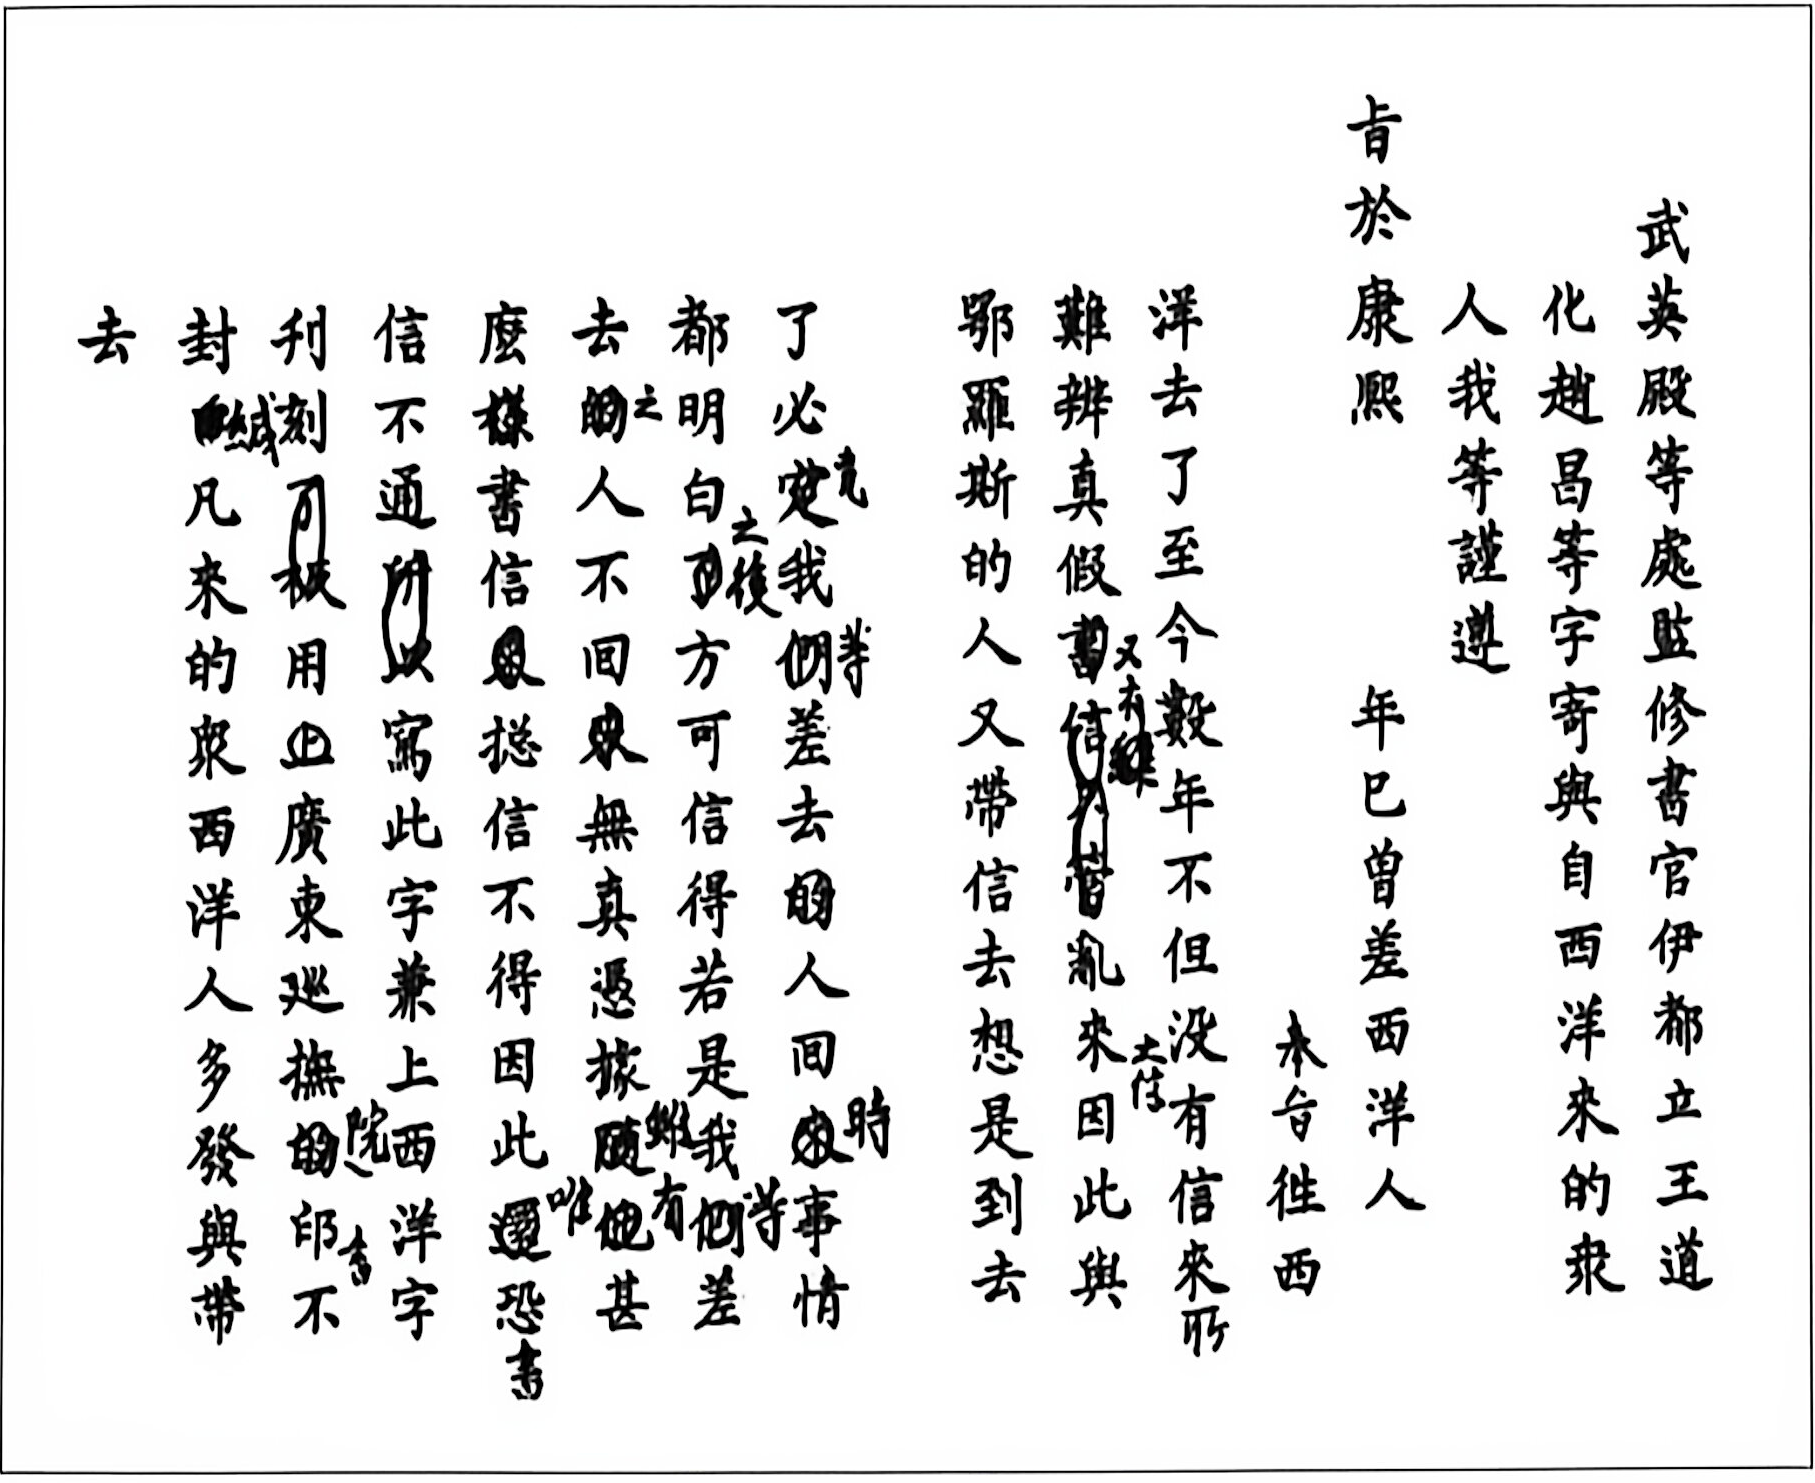
\includegraphics[width=\linewidth,height=.76\textheight,keepaspectratio]{assets/figures/kangxi-red-ticket-draft.png}
\caption*{图0.1\quad 康熙御批红票草稿}
\BookFloatNotes{图片来源：陈垣编，《康熙与罗马使节关系文书》，文件9。}
\end{figure}%
瑟四位西洋人都是来华的传教士，清代官修史书中并没有提到过这%
四人出使西方，他们到底是以什么身份被康熙派出的？红票中只说%
四人是被“差”去西洋，是“奉旨往西洋去了”。同时，红票中的拉%
丁文翻译，写的也是被皇帝派往欧洲，没有给出一个名号。龙安国%
原名 Antonio de Barros，是葡萄牙人；薄贤士原名 Antoine de Beauvol-%
lier，是法国人。二人去欧洲时选择跨越太平洋，走的是美洲路线，到%
达巴西后还给欧洲寄过信，但后来二人在从巴西去欧洲的路上遇到%
风暴，死在了途中。艾若瑟原名 Giuseppe Provana，是意大利人；陆%
若瑟原名 José Raimundo de Arxo，是西班牙人。这二人走的是印度洋%
路线，最后都到达欧洲，还受到了葡萄牙国王的热情接待。陆若瑟%
到达欧洲不久后就病故了。在红票传到欧洲时，只有艾若瑟还活着。%
教皇看到红票以后，批准艾若瑟返回中国。可惜艾若瑟在回程的船%
上去世了。艾若瑟离开中国的时候，还带了一个中国弟子，叫樊守%
义。他一直跟着艾若瑟在欧洲游历，最后守着艾若瑟的棺材抵达广%
州。康熙后来派人去广州，买了36亩土地用作墓地，风光厚葬了艾%
若瑟。当然这段厚葬的历史，清史中也没有记载。艾若瑟的墓早已%
被毁，现在只有一些大理石墓碑残片，存于广州市博物馆中。好在%
19世纪后期，艾若瑟的墓地是当时洋人爱去的一个景点，一位行经%
此处的英国人在游记中详细记录了墓地的情况，还把当时墓碑和墓%
志铭上的拉丁文和汉文全部抄录了下来。在这份抄录中，我们可以%
看到艾若瑟的墓碑正面，刻出的是“钦差艾公之墓”，也就是说康熙%
赐给艾若瑟的名头是“钦差”。艾若瑟的墓碑上还有长篇墓志铭，记%
录下了康熙派内务府人到广州操办墓地的事，同时还比照《汉书·苏%
武传》，赞美了艾若瑟“钦差大西洋公干”而滞留海外十三载后，不%
虑“波涛险幻，坚为复命”的美事。盖棺而后论定，这四位来华的%
欧洲传教士在康熙心中，都是他的“钦差”。%
\par
% 原书页码：vii–viii；段落（跨页续段）
为什么大清皇帝会派洋人做自己的“钦差”出访？这些传教士和%
康熙是什么关系？他们为什么能得到康熙的信任？这些都是本书要探%
索的问题。红票的拉丁文下面，还有十六位来自欧洲各国的在京传教%
士，为康熙发出的红票签名，确认红票内容的真实性。%
% 原书页码：vii；图表（图题／表题所在页）
% 原书页码：vii；表格、表题与表注共用一个环境。
\begin{table}[!htbp]\phantomsection\label{table-16}
\centering\BookTableStyle
\begin{tabularx}{\linewidth}{|>{\raggedright\arraybackslash}X|>{\centering\arraybackslash}p{18mm}|>{\centering\arraybackslash}p{20mm}|>{\centering\arraybackslash}p{18mm}|}
\hline
英文拼写 & 中文名 & 入华时间 & 国家 \\ \hline
Matteo Ripa & 马国贤 & 1710 & 意大利 \\ \hline
Teodorico Pedrini & 德里格 & 1711 & 意大利 \\ \hline
Kilian Stumpf S. J. & 纪理安 & 1694 & 德国 \\ \hline
Joseph Suarez S. J. & 苏霖 & 1684 & 葡萄牙 \\ \hline
Joachim Bouvet S. J. & 白晋 & 1687 & 法国 \\ \hline
Jean-François Foucquet S. J. & 傅圣泽 & 1699 & 法国 \\ \hline
Dominique Parrenin S. J. & 巴多明 & 1698 & 法国 \\ \hline
Pierre Vincent de Tartre S. J. & 汤尚贤 & 1701 & 法国 \\ \hline
Pierre Jartoux S. J. & 杜德美 & 1701 & 法国 \\ \hline
Jean Francisco Cardoso S. J. & 麦大成 & 1710 & 葡萄牙 \\ \hline
Joannes Mourao S. J. & 穆经远 & 1710 & 葡萄牙 \\ \hline
Giuseppe Baudino S. J. & 鲍仲义 & 1694 & 意大利 \\ \hline
Frantz Stadlin S. J. & 林济各 & 1707 & 瑞士 \\ \hline
Jacobus Brocard S. J. & 陆伯嘉 & 1701 & 法国 \\ \hline
Joseph da Costa S. J. & 罗怀忠 & 1715 & 意大利 \\ \hline
Joseph Castiglione S. J. & 郎世宁 & 1715 & 意大利 \\ \hline
\end{tabularx}
\end{table}%
%
这些签名的传教士和康熙又是什么关系？康熙和传教士关系密切并不%
是什么秘闻，当年传教士在寄回欧洲的信中经常炫耀他们和康熙的关%
系，以至于有些欧洲人燃起了一丝希望：康熙有没有可能成为第二个%
君士坦丁大帝（罗马第一个接受基督教的皇帝）？%
\par
% 原书页码：viii；段落
从中国的政治史角度看，康熙和传教士的关系也很特殊。大部分%
传教士都没有官衔，却能往来于宫中，侍奉在康熙左右。紫禁城按功%
能分为内廷和外廷。大臣上朝议事，处理公务都在外廷；内廷算是皇%
帝的私人领域，是皇帝生活起居与日常办公的地方。让当时朝臣都羡%
慕的是，传教士被康熙允许出人内廷。尽管有几个传教士在朝廷也有%
过官衔，负责天象观测这种技术活儿，但按理他们都是不能出人内廷%
的。出入紫禁城从来不是件容易的事，更不要说日常出现在皇帝身边。%
以前的研究者大多都认为，传教士能在康熙左右，是因为康熙对西学%
感兴趣，传教士对他有用处。这种说法颠倒了先后关系。兴趣源自接%
触，康熙对西方学问的兴趣，是不可能凭空产生的。古往今来，能长%
时间接触到皇帝，先决条件都是信任。所以先后顺序应该是，康熙先%
有了对传教士的信任，才会有和他们的接触，从而他们才有机会教康%
熙西方的学术和技术。只有康熙学习了这些知识以后，他才能对西学%
有兴趣，也才能理解传教士那些学问的用处所在。%
\par
% 原书页码：viii–ix；段落（跨页续段）
康熙对传教士的信任，不仅仅体现在让他们出入紫禁城，派他们%
去欧洲，甚至连跟俄罗斯的边界谈判这样核心的国家事务，他也派出%
了两位传教士加人到谈判队伍中。著名的1689年中俄《尼布楚条约》，%
就是两位传教士作为清朝的实际谈判代表，和俄罗斯人谈出来的。双%
方会谈语言是拉丁语。最后的合约由拉丁文、满文和俄文三种语言签%
订，没有汉文。传教士在谈判中说着拉丁文但又忠于清朝，这让俄罗%
斯谈判代表很吃惊，而且他们发现传教士坚决捍卫清朝利益，比以前%
谈判过的满人还要强硬。最后签订的条约，彼得大帝不满意，而且对%
传教士竟然帮助异教徒谈判很不理解，一怒之下，把两位传教士所属%
的耶稣会给禁了，不允许任何耶稣会的传教士进入俄罗斯。%
\par
% 原书页码：ix；段落
在北京的传教士，大多都属于耶稣会。耶稣会1540年成立于欧%
洲。在环球航海的大背景下，耶稣会立会的一个宗旨就是要把天主%
教传播到世界各地，这一点得到了罗马教皇的支持。该会七大创始人%
之一圣方济各·沙勿略（St. Francis Xavier）早在 1551年就远渡重洋，%
来到了广东外面的岛屿，准备找机会进入中国。后来著名的利玛窦神%
父，也是耶稣会传教士，他是在万历年间进人的中国内陆。之后陆续%
到达的耶稣会神父一直孜孜不倦地探索如何融入中国的士大夫圈子，%
在中国传播他们的福音。耶稣会神父在江南成功进入了一些文人圈%
子，同时也为一些当时的名人施洗人教。明朝末年，耶稣会神父汤若%
望进入了朝廷体制，在明朝的钦天监做官。当时他在京城与朝野士人%
多有结交。%
\par
% 原书页码：ix–x；段落（跨页续段）
明清易代之际，在华传教士跟当时所有国人一样经历了战争的痛%
苦。对他们来说，朝代更替也是一次机会，一个让他们走进统治阶层%
权力圈子的机会。传教士从最初见到进京的多尔衮，到后来的顺治皇%
帝，再经历鳌拜专权，最后走进康熙的世界。在康熙的孩提时代，传%
教士就在他身边。在康熙跟着翰林们学习汉语和经史子集的同时，传%
教士在内廷里教他数学等西方学问。传教士后来又一步步地帮助康熙%
和欧洲建立起了各种联系，同时也让欧洲对这个东方皇帝产生了兴趣。%
莱布尼茨、伏尔泰等欧洲科学家和哲学家都在饶有兴致地阅读康熙的%
传记。红票正好是全球化之初中西交流中留下的一页。大概也是近年%
中外历史学界对这段历史的挖掘，让红票的历史位置日渐清晰，拍卖%
中的红票，一路竞价，最后以161万成交。%
% 原书页码：无印刷页码；卷首插图，图1原件漏扫，其完整图注见扫描020。
% 用户于2026-10-12确认缺图为康熙坐像。以故宫藏《康熙帝读书像》高清公开图补入。
% 图像来源：https://commons.wikimedia.org/wiki/File:康熙帝读书像轴.jpg
% 馆藏说明：https://www.dpm.org.cn/collection/paint/230329.html
\par
\begin{figure}[p]\phantomsection\label{fig-front-kangxi}
\centering
% 原文件保持完整；排版时仅裁去右侧拍摄色卡边缘（70像素）。
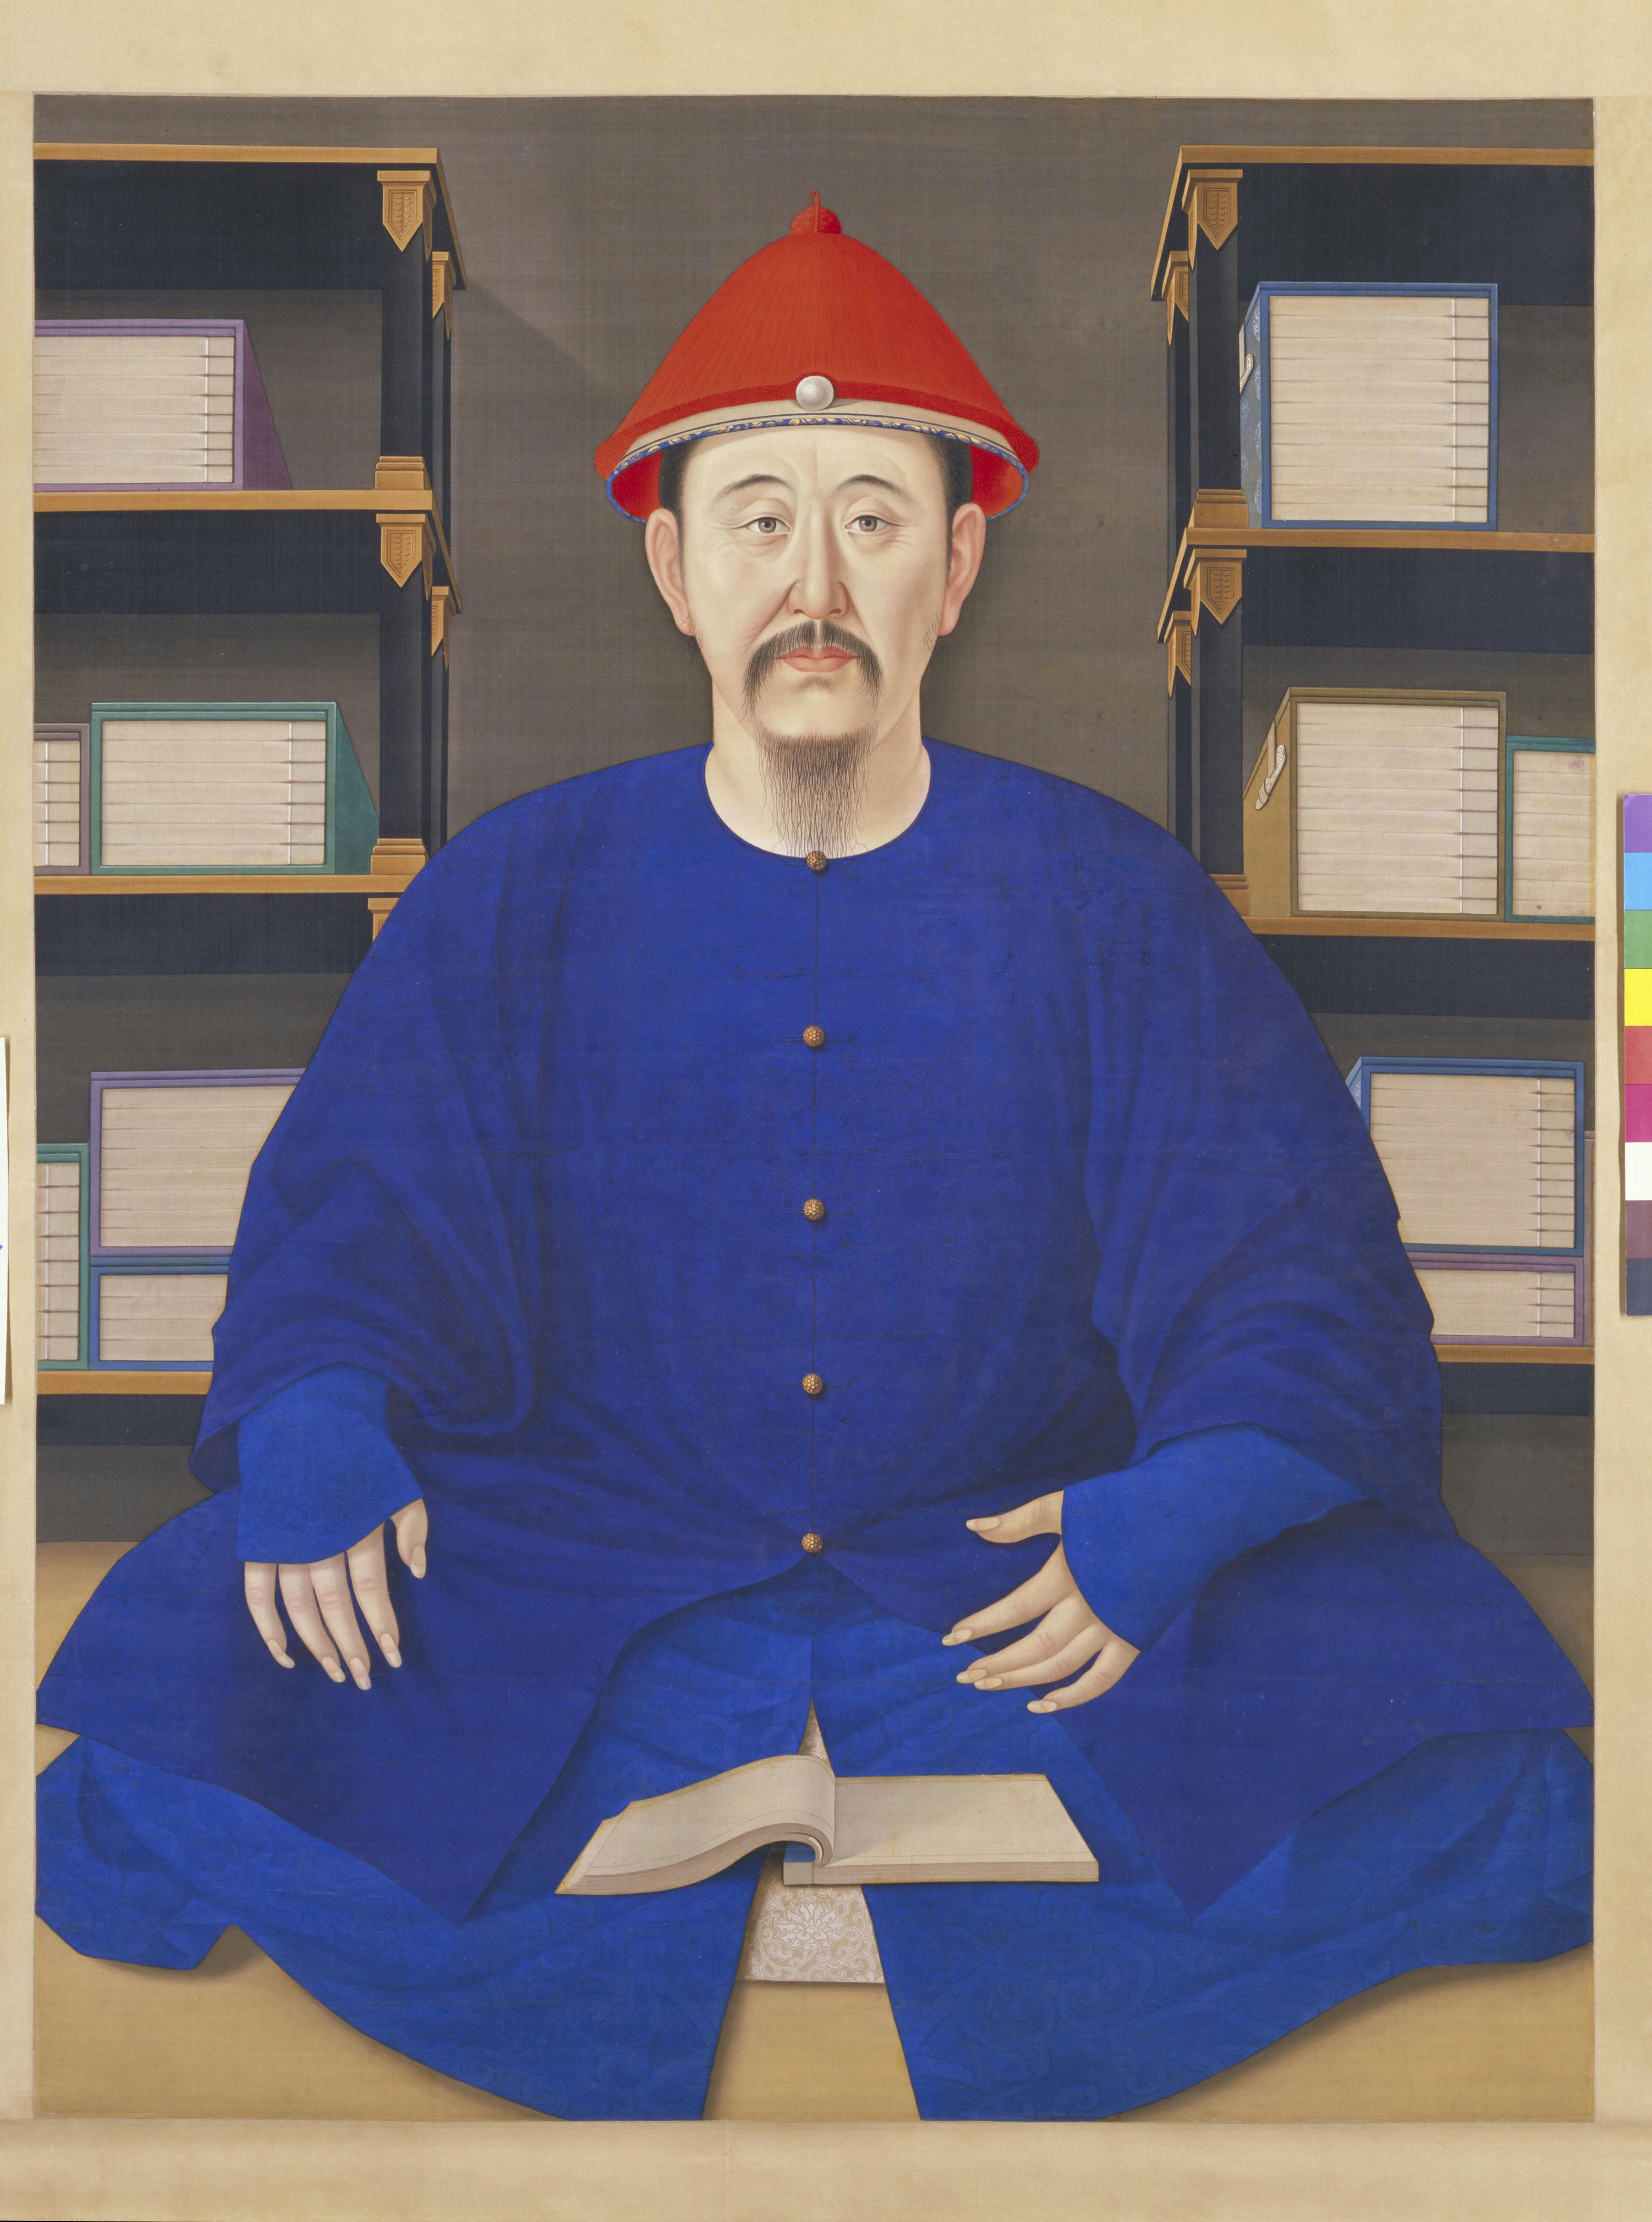
\includegraphics[width=\linewidth,height=.76\textheight,keepaspectratio,trim=0 0 70bp 0,clip]{assets/figures/kangxi-reading.jpg}
\caption*{图1\quad 康熙坐像，故宫博物院藏。画中人物和书架的透视关系以及后面的阴影都是典型的西洋画技法，展现出全球化之初中西文化的互动。}
\end{figure}%
% 原书页码：无印刷页码；卷首图2与图注见扫描020。
\begin{figure}[p]\phantomsection\label{fig-front-tapestry}
\centering
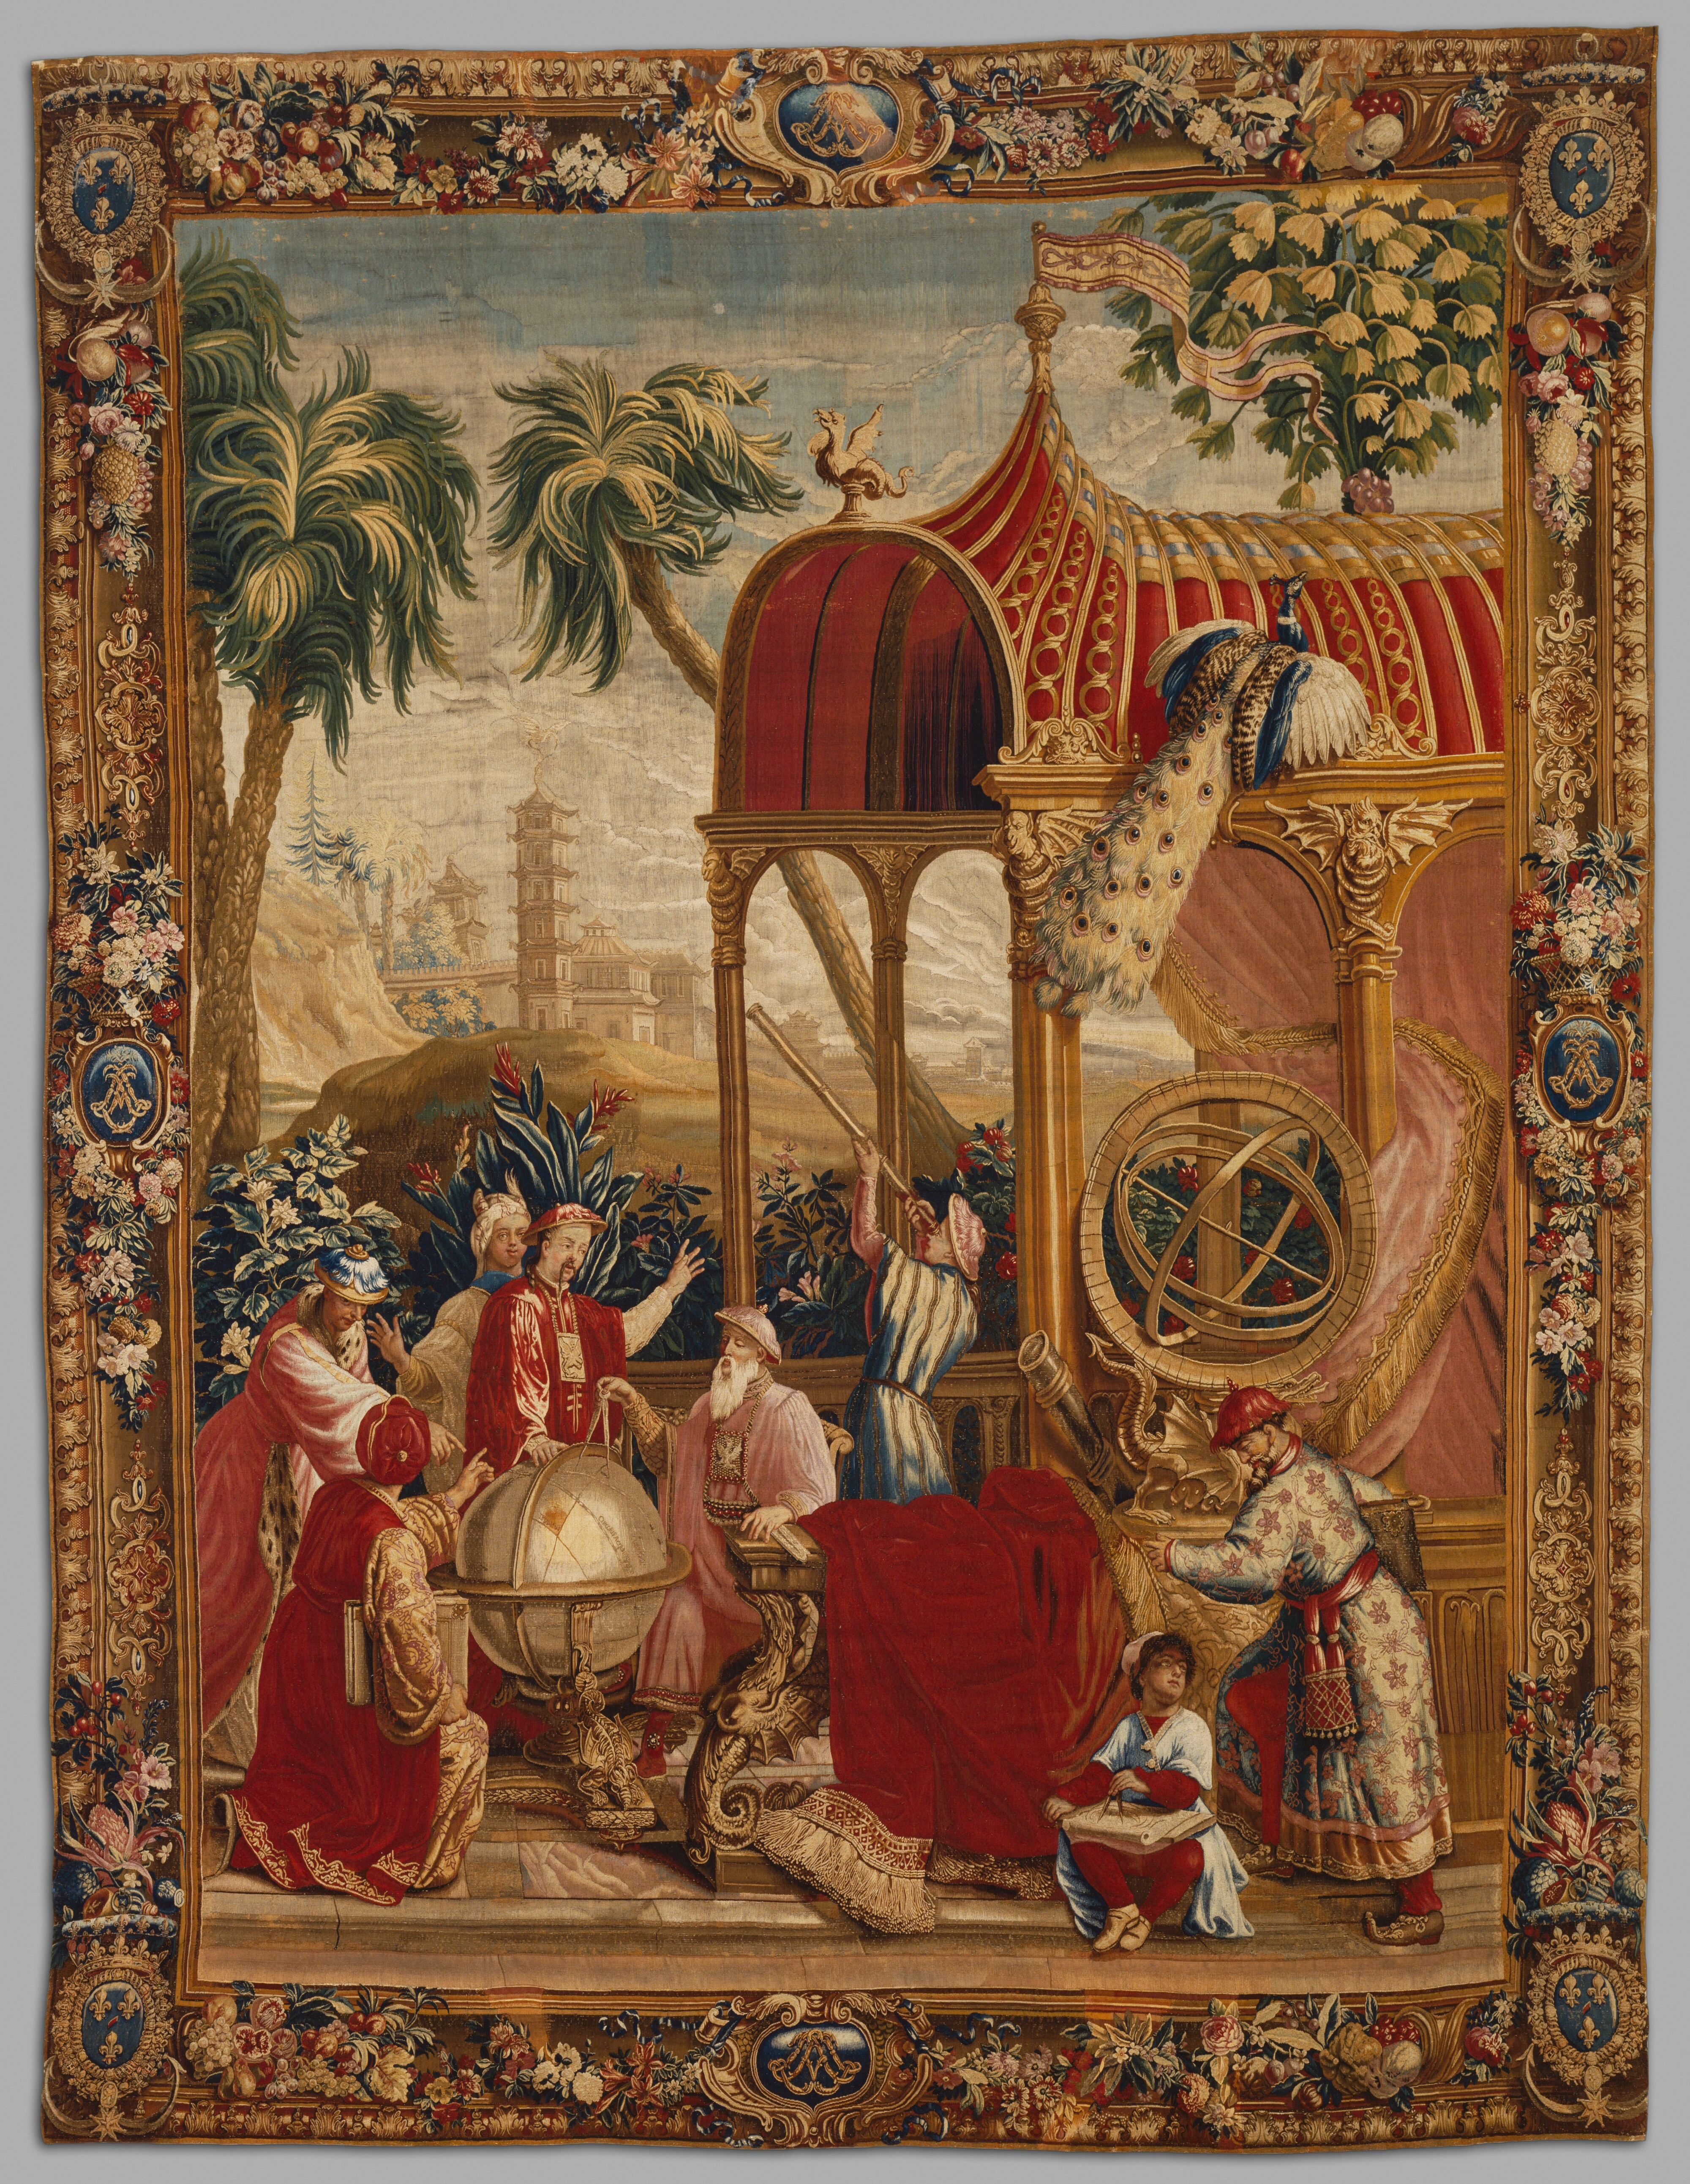
\includegraphics[width=\linewidth,height=.76\textheight,keepaspectratio]{assets/figures/emperor-tapestry.jpg}
\caption*{图2\quad “中国皇帝外出巡幸”挂毯。尺寸：254×415.3cm，产地：法国，年份：1697—1705。盖蒂博物馆藏。挂毯图案为根据入华传教士写回欧洲的信件中关于中国皇帝的故事而想象创作。}
\end{figure}%
